\documentclass{article}

\usepackage{amsbsy,amscd,amsfonts,amsgen,amsmath,amsopn,amssymb,amstext,amsthm,amsxtra}
\usepackage{graphicx}
\usepackage{verbatim}
\usepackage[utf8]{inputenc}

%-------------------------------------------------------------------
% You can insert user-defined macros 
\DeclareUnicodeCharacter{03B2}{\beta}
%-------------------------------------------------------------------

\title{Multiplication of Signed Binary Numbers in Computer Hardware: A Constructivist Approach}
\date{\today}
\author{Christopher Jenkins\\ Trinity University, cjenkin1@trinity.edu
    \and Adam Voss\\ Luther College, vossad01@luther.edu}

\begin{document}

\maketitle
\tableofcontents

\pagebreak

\section{Objectives and Preparation}
In this text we will introduce the concept of multiplication of signed binary numbers and work towards a simple but relatively efficient multiplication algorithm known as Booth's Multiplication Algorithm.
To follow this text you will need to be familiar with two's complement representation of singed binary numbers.
We will use big-endian ordering for these numbers, meaning the right most bit (bit 0) will be the least significant bit of the number.

Some background on machine architecture, such as an understanding of registers and primitive operations, will also be helpful.

We recommend this text be used in conjunction with the Booth’s Multiplication Algorithm Visualization available on the Java-Hosted Algorithm Visualization Environment (JHAVE).
For information regarding the use of this tool, consult ``A Guide for Visualizing Booth’s Multiplication Algorithm''.
%add URL here

\section{Multiplication by Repeated Additions}
Multiplication is often defined as repeated additions, like so: \begin{align}
a \cdot b = 0 + \underbrace{a + \cdots + a}_{b} %TODO cite Wikipedia!
\end{align}
Thus, to calculate $11 \times 23$, you would start with 0 and add 11 to it 23 times.

This method works equally well for binary numbers: %This might flow better if I didn't go back and forth between Binary, Decimal
\begin{equation}
1111 \cdot 0011 = 0 + 1111 + 1111 + 1111 = 1101
\end{equation}

Despite working for multiplying signed numbers, this method has the undesired characteristic of having varying execution time since it is tied to the magnitude of the numbers being multiplied.
For example, the equivalent problem of calculating $23 \times 11$ requires twelve fewer operations.
You could first make a comparison to ensure that you always multiply by the smaller number, but on average there will still be many additions.
Computer architects generally prefer predictability in execution times, and since we do not usually do repeated additions when we multiply decimal numbers by hand anyway, we should hope that we can find some insight from our experience of doing decimal multiplication to find a more efficient and predictable way to do binary multiplication with hardware.

%This section seems math-y, maybe should be re-arranged in the article
\section{Multiplication using the `Shift-and-Add' Method}
The ``shift-and-add'' method for binary multiplication is the same as multiplication by partial products, which is the method most people use to do long multiplication.
To review, multiplication by partial products involves multiplying one number, called the multiplicand (or $M$), by successively more significant digits of the other number, called the multiplier (or $Q$).%Consistancy!
Each of these individual multiplications is referred to as a \textsl{partial product}.
The sum of all the partial products is the product of $M$ and $Q$.

%This paragraph is very much draft quality, but I thought it important to show where the name came from
% as this provides more background as well at introducing hardware for parity with how we present Booth.

%If this is not what you wanted for shift and add, then maybe present it as partial products
%Then use the next section to provide how partial products translates to shifts and add in HW

Another way to think of this is as follows: let $Q$ be an n-digit binary number and let the $i^{th}$ bit of $Q$ be denoted $q_i$ (this text goes by the convention that the $0^{th}$ bit of a binary value is the rightmost or least-significant bit).
Then the significance (or ``place-value'' as you learned it in elementary school) of $q_i$ is $2^i$.
We can then express the problem $M \times Q$ as $M \times (q_{n-1} \times 2^{n-1} + q_{n-2} \times 2^{n-2} + \ldots + q_{0} \times 2^{0})$.
Each one of the products $(q_i \times 2^{i}) \times M$ is a partial product.
For binary values, there are only two values a partial product may be: if $q_i = 0$, then the result is simply $0$; otherwise the result is $M \times 2^i$.

Consider the following calculation of the multiplication of 001011 and 010111, which are the numbers 11 and 23 in two's complement notation, respectively.
Since many computer architectures use fixed-sized registers to hold data, we will use the same number of bits to represent both $M$ and $Q$.

%diagram goes here
\begin{figure}[h]
\centering
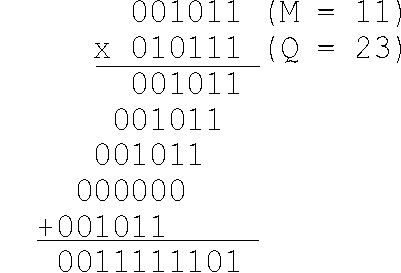
\includegraphics[scale=0.7]{saam3.pdf}
\caption{Shift-and-Add Method}
\end{figure}

We see already an improvement in the performance of this algorithm, compared to the repeated additions method.
Each partial product shown corresponds to an addition operation (+M or +0).
In every line except the first, there is also an implicit shift operation, corresponding to the significance of the bit being multiplied with $M$.
Again, recall that the significance of bit $q_i$ is $2^i$, so if $q_i = 1$, then the partial product looks like $M$ followed by $i$ trailing 0s.
Much like multiplying by powers of $10$ in decimal, we are simply ``shifting'' the bits in M to more significant place values.

Compare the method described above, which involves the addition of 5 partial products and 4 shifts for this problem, to the method proposed in the introduction, which requires 23 additions.
Even though this is only one example, it should give you a good idea of how much better the performance of this algorithm is than the first.
The speedup is even greater if one considers that, on some machines, shift operations can potentially take less time than addition operations.

\pagebreak

\section{Improving the Shift-and-Add Method}
There are several issues that prevent us from directly implementing the shift-and-add algorithm in hardware.
To begin with, most ALUs are only capable of adding two numbers together at a time.
This means a \emph{running product} must be calculated for every partial product, instead of calculating the final product at the very end of the process.
The running product is initialized to 0, and for every partial product calculated the new running product is the sum of the old running product plus the partial product.
We will call the space used to store the running product register A.
Since we are beginning our discussion of computer design problems, we will similarly refer to the space used to store the multiplicand and multiplier as register M and register Q, respectively.

Notice also that, as the algorithm progresses, the position at which the numbers are added incrementally slides to the left.
It is a much simpler task to always add into the same location of the running product and then shift the running product to the right by 1.
We refer to this operation as a \emph{sign-preserving right shift}; it is also known as an \emph{arithmetic right shift}.

Finally, we need to consider register size.
In the previous example, the numbers we multiplied were represented as 6-digit binary values; their result, however, required 10 bits to represent.
In general, if two n-bit numbers are multiplied, then the result can require as many as 2n bits to represent.
Thus, the convention is to store the result of multiplication between two registers.

Figure 2 depicts an execution of the shift-and-add multiplication algorithm which addresses the problems we have so far considered.
You should study it.

\begin{figure}[h]
\centering
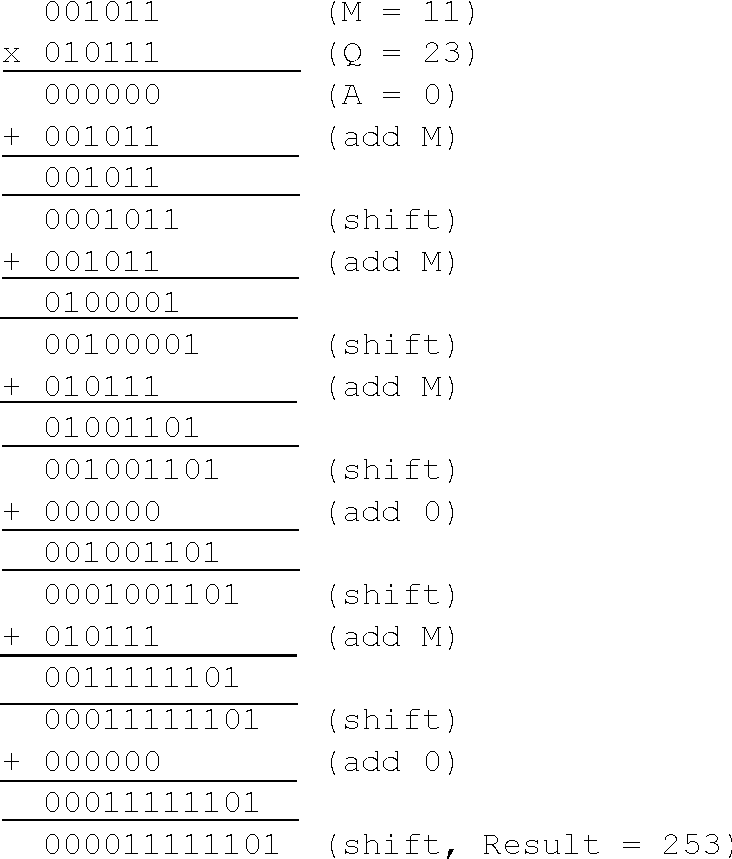
\includegraphics[scale=0.7]{isaam2.pdf}
\caption{Improved Shift-and-Add Multiplication}
\end{figure}

\pagebreak

There is still another computer design issue which could make this method easier to implement in hardware: in the last example, the bit in register Q we are using to calculate a partial product is always positioned one to the left of the previous bit we used, or else it is the right-most (least significant, \emph{lsb}) bit of register Q when the multiplication starts.
We could instead choose to always examine the \emph{lsb} of register Q, and for every right shift operation on register A, we would also do a right shift on register Q.
This means that as the algorithm progresses, the value in Q is discarded one bit at a time.%Thus, when the algorithm finishes, all of the previous values in Q will have been discarded.
This will allow us to be even more efficient: instead of using another register to store the lower half of the product, we can use register Q, because, for every bit discarded from Q, we can place into Q's most significant bit (\emph{msb}) the \emph{lsb} of A, saving ourselves from using a whole other register!

\begin{figure}[h]
\centering
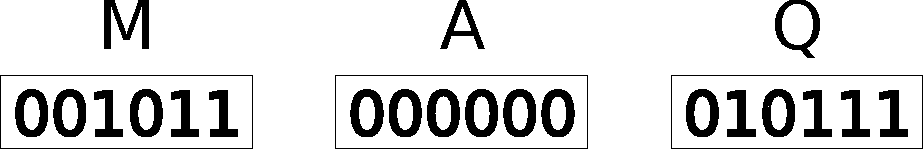
\includegraphics[scale=0.4]{init.pdf}
\caption{Registers M, A, and Q, initialized for the multiplication of 11 and 23}
\end{figure}%TODO why doesn't this print? Try another figure

\pagebreak

\section{The Problem with Negative Numbers}
Consider the multiplication of the following 4-bit two's complement numbers: 0011 (3) and 1011 (-5).
We expect a result of -15 (11110001); however, currently the method we have been developing is unable to distinguish between signed and unsigned values, and would multiply 3 by 11 (the unsigned decimal value of 1011).
In this case, we must calculate the absolute values of the numbers before multiplying them.
When we are finished, we determine the sign of the result in the same way we would with decimal multiplication:
%One way around this behavior would be to calculate the absolute values of our multiplier and multiplicand.
%Then, after the positive product was calculated, if either the multiplicand or the multiplier are negative (but not both), calculate the two's complement of the product.

\begin{center}
    \begin{tabular}{| l | l | l |}
        \hline
        multiplicand & multiplier & product \\
        \hline
        positive & positive & positive \\
        positive & negative & negative \\
        negative & positive & negative \\
        negative & negative & positive \\
        \hline
    \end{tabular}
\end{center}

This is a suboptimal solution from a design point of view, as it introduces the need for extra hardware and/or processing of binary numbers whenever we wish to multiply.

\section{Booth's Encoding}
In 1951, Andrew Booth introduced an alternative method for multiplying two's complement numbers.
At its heart is the observation that a number like 0111, which is understood to mean $2^2 + 2^1 + 2^0 = 4 + 2 + 1 = 7$, can also be thought of as $2^3 - 2^0 = 8 - 1 = 7$.
This can be written (encoded) as $100\bar{1}$, where 1 and 0 have their understood meanings, and $\bar{1}$ represents $-1$.
Generally, it can be shown that any sequence $2^n + 2^{n-1} + ... + 2^{n-k}$ (where $k+1$ is the number of terms in the sequence) is equal to $2^{n+1} - 2^{n-k}$.

To encode an $n$-digit binary number $m$, examine the $i^{th}$ digit of $m$ (we will call this digit $m_i$) and do one of the following: %TODO citation needed for this

\begin{enumerate}
\item If $m_i$ and $m_{i-1}$ (the digit to the right of $m_i$) are 1 and 1, or they are 0 and 0, write 0 at the $i^{th}$ digit in the new encoded value.
\item If $m_i$ and $m_{i-1}$ are 0 and 1 respectively, write 1 at the $i^{th}$ digit in the new encoded value.
\item If $m_i$ and $m_{i-1}$ are 1 and 0 respectively, write $\bar{1}$ at the $i^{th}$ digit in the new encoded value.
\item When $i = 0$, assume $m_{i-1}$ is 0
\end{enumerate}

Take for example the binary number 011100011, which is $2^7 + 2^6 + 2^5 + 2^1 + 2^0 = 227$.
Applying the method described above, our encoded value for this number is $100\bar{1}0010\bar{1}$ which is $2^8 - 2^5 + 2^2 - 2^0 = 227$
In this way, the method takes a ``run'' of $1$s in a binary value (representing the series $2^{n} + 2^{n-1} + ...
+ 2^{n-k}$), takes the first 0 bit to the left of the run and turns it into $1$ and turns the entire run into $0$s except for the last $1$ in the run, which is turned into $\bar{1}$.

How does this solve the problem of negative numbers?
Remember that in a two's complement binary value the \emph{msb} represents a subtraction of the highest power of two.
For example, $11100100$ represents the value $-(2^{7}) + 2^{6} + 2^{5} + 2^{2} = -128 + 64 + 32 + 4 = -28$.
Applying the method described above, we obtain an encoded value of $00\bar{1}01\bar{1}00$, which represents $-(2^{5}) + 2^{3} - 2^{2} = -32 + 8 - 4 = -28$.
Generally, if the \emph{msb} of an n-digit two's complement binary number is 1, then the leftmost ``run'' of $1$s represents the value $-(2^{n-1}) + 2^{n-2} + ...
+ 2^{(n-1)-k}$.
Using the mathematical insight of Booth's Encoding technique, we convert this to $-(2^{n-1}) + (2^{n-1}) - 2^{(n-1)-k} = -2^{(n-1)-k}$.
(Our sequence in this case was $2^{n-2} + 2^{n-3} + ...
+ 2^{(n-1)-k}$)
Because Booth's Encoding is based on this mathematical equivalence, we are guaranteed to preserve the value of the candidate number, whether positive or negative.
 
%TODO this belongs in hardware discussion
%This property has the potential to further increase efficiency, as any arbitrary ``run'' of $1$s (series of powers of 2) will be reduced to just 2 arithmetic operations, since when we encounter $0$s we need only shift.

\section{Booth's Algorithm in Hardware}
    At the hardware level we are only allowed the use of 0 and 1 to represent values, so we instead examine pairs of bits.
Scanning a binary number from right to left, the pair `10' signifies the beginning of a sequence of 1s and thus corresponds to a subtraction (or $\bar{1}$).
The pair `01' signifies the end of a sequence of 1s and corresponds to an addition.
The pairs '00' and '11' signify that no arithmetic operations need occur (the equivalent of adding 0).
This property has the potential to increase the efficiency of our algorithm, as any arbitrary ``run'' of $1$s will be reduced to just 2 arithmetic operations.

Since we would like to stay as close as possible to the algorithm outlined earlier, all cases will still require a shift.

    In order to examine pairs of bits, we add an extra 1 bit register, called $\beta$ (or Beta) to hold the bit shifted out of register Q.
$\beta$ is initialized to 0, so that at the start of the algorithm, if the least significant bit of Q is 1, the computer will read a pair `10' and execute a subtraction.
Keep in mind now that whenever a shift occurs, the least significant bit of A is moved into the most significant bit of Q, and the least significant bit of Q is moved into $\beta$.
The old value of $\beta$ is discarded.

\begin{figure}[h]
\centering
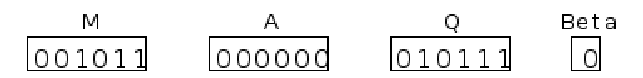
\includegraphics[scale=0.4]{init2.pdf}
\caption{Registers M, A, Q, and Beta, initialized for the multiplication of 11 and 23}
\end{figure}%TODO FIGURE

\pagebreak

\section{Visualizing Booth's Multiplication}
Everything we have considered so far for an appropriate machine level algorithm to multiply two's complement values has been implemented as a JHAVÉ algorithm visualization.
Instead of using the form of the previous examples, it more closely resembles the way the algorithm might be executed in hardware, placing explicitly the multiplicand and multiplier in registers M and Q respectively, and storing the final result in registers A and Q.
Familiarize yourself with the format of the visualization by consulting ``A Guide for Visualizing Booth’s Multiplication Algorithm'', then step through the visualization as many times as you need to understand how the algorithm works, answering the questions as they appear.
Once you have finished, proceed to the exercises, detailed below.

\section{Exercises}
For each of the following exercises, there is a corresponding visualization with the same name available on JHAVÉ.
We suggest solving the exercises by entering your answers into the visualization's ``input generator'', as the visualization is designed to judge the correctness of your solution and provided feedback if you have made a mistake.

\begin{description}
    \item [Exercise 1] Initialize Booth's Multiplication Algorithm for the multiplication of two random integers X and Y by giving the values of the registers M, A, and Q, the bit $\beta$, and Count
    \item [Exercise 2] Complete Booth's Multiplication Algorithm for the multiplication of two random integers X and Y by initializing the values of the registers M, A, Q, the bit $\beta$, and Count, and then giving the values of each at the end of each iteration of the algorithm's loop
    \item [Exercise 3] Give numbers X and Y, either in binary or in decimal, so that they will result in the least efficient performance of Booth's Algorithm for $n$-digit binary numbers, i.e. those $n$-digit binary numbers which will result in the greatest number possible of both arithmetic and shift operations combined
\end{description}
%For your reference, the previous states of the registers are kept on screen as the visualization progresses.
%They are grayed to indicate they are no longer the active values of the registers.
%An example run-through is provided below, as well as a link to a use-case video.%TODO this
%Step through the visualization as many times as you need, answering the questions as they appear, then proceed on to the exercises.

%\section{Example Run of the Visualization}
%After starting the JHAVÉ client and selecting ``Booth's Multiplication Algorithm'', an input generator window will appear with four text fields, two for decimal input and two four binary input, and a menu to select register size.
%You may choose your own values for the visualization, or use the default values provided (if you are having trouble getting the input generator to take your values, make sure you selected an appropriate register size for your values).
%When you are ready to begin the visualization, press ``OK''.

%\begin{figure}[h]
%\centering
%\includegraphics{vis1.pdf}
%\end{figure}

%The next few snapshots of the visualization 

%\section{How it works}
%-------------------------------------------------------------------
% to create references, un-comment \bibliographystyle{plain} and
% un-comment \bibliography{myBIBfile} and re-name its arguemnt(s)
% to point at the .bib file(s) containing the BibTeX references:

%\bibliographystyle{plain}
%\bibliography{myBIBfile}

\end{document}
